\documentclass[11pt]{amsart}
\usepackage{geometry}                % See geometry.pdf to learn the layout options. There are lots.
\geometry{letterpaper}                   % ... or a4paper or a5paper or ...
%\geometry{landscape}                % Activate for for rotated page geometry
%\usepackage[parfill]{parskip}    % Activate to begin paragraphs with an empty line rather than an indent
\usepackage{booktabs}
\usepackage{graphicx}
\usepackage{amssymb}
\usepackage{epstopdf}
\usepackage{caption}
\usepackage{subcaption}
\usepackage{commath}
\DeclareGraphicsRule{.tif}{png}{.png}{`convert #1 `dirname #1`/`basename #1 .tif`.png}

% Declare commands
\newcommand{\mat}[1]{\mathbf{#1}}

\title{CS 181 -- Practical 2}
\author{Casey Grun, Sam Kim, Rhed Shi}
%\date{}                                           % Activate to display a given date or no date

\begin{document}
\maketitle

\section{Warmup}

\section{Regression algorithms}

Our challenge was to predict movie revenues for a set of movies from available data about the movies. We first transform each piece of data about each of the movies into some feature vector $x_i$, and then we concatenate the features from the $N$ movies into a feature matrix $X$. We are given the opening revenues for each movie in a column vector $y$. Predicting revenues thus amounted to solving the regression problem
$$\min_w \frac{1}{N}\sum |X w - y|$$
That is, given some $N \times D$ feature data matrix $X$, an $N \times 1$ target matrix $y$, we needed to produce a set of feature weights $w$; then given some new test data $X'$, we can predict the revenues for this data by $\hat{y} = X' w$. Our challenge is therefore to determine the optimal transformation from a movie into a feature vector $x_i$ and the optimal method of solving the above regression problem to determine $w$. 

\subsection{LSMR and LSQR}

Both the LSQR and LSMR algorithms solve the linear system $Ax=b$, or $\text{min}\norm{b-Ax}_2$ if the system is inconsistent, for sparse matrices $A$ \cite{LSMR}. For regularization (Ridge regression), these algorithms solve $\text{min}\norm{b-Ax}^2+\lambda^2\norm{x}^2$ where $\lambda$ is the damping parameter. In our example, $A$ is the feature matrix, $x$ is the weights, and $b$ is the vector of predicted revenues. Given $A$ and $b$ from the feature extraction modules on the training data, we want to solve for $x$ so that we can predict the revenues on test data after extracting the feature matrix from the test data.

Assuming that we are solving for the non-regularized least squares (the results are easily generalized to regularized least squares), LSQR uses conjugate-gradient to the equation $(A^TA+\lambda^2I)x=A^Tb$, which has the property of reducing $\norm{b-Ax_k}$ monotonically. LSMR, on the other hand, uses MINRES to the equation $(A^TA+\lambda^2I)x=A^Tb$, which has the property of reducing both $\norm{b-Ax_k}$ and $\norm{A^T(b-Ax_k)}$ monotonically. Because of these properties, although both LSQR and LSMR converge to similar points, LSMR converges more quickly and can reach a more accurate answer. This suggests that it may be possible to reach a similar result using LSQR but with tighter termination tolerances.

The LSMR algorithm using default parameters ($\lambda=0$) shows a significant improvement in MAE of $7.7\times10^5$ on the Kaggle data.

\subsection{Regularization for LSMR}
Because of the large number of features, especially those extracted from the reviews (see below sections on feature extraction), we must be careful about overfitting to the limited data. Regularization can alleviate this problem, and the LSMR algorithm performs algorithm by solving $\text{min}\norm{b-Ax}^2+\lambda^2\norm{x}^2$ where $\lambda$ is the damping parameter. Cross-validation on the same subset of the training data revealed the optimal damping parameter to be around $\lambda=15000$, which decreased the MAE by approximately $17000$. Further increasing $\lambda$ causes the MAE to shoot up significantly, consistent with the bias-variance decomposition analysis presented by Bishop in Figure 3.6. The below figure shows a plot of the MAE on the subset of training data as a function of $\log{\lambda}$.

\begin{center}
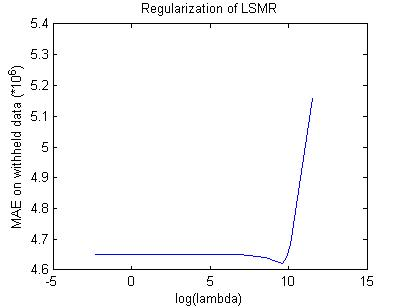
\includegraphics[width=10cm]{LSMR-Regularization.jpg}
\end{center}

\subsection{Basis functions}
Solving $Ax=b$ for $x$, the weights, places the restriction that the revenues, $b$ depend only linearly on all of the features, and does not account for possible non-linear dependencies. We thus implemented a polynomial basis for each feature ($\phi_j(x)=x^j$). In this scheme, if $A$ is originally a $n\times m$ matrix, then it is extended to an $n \times mB$ matrix, where $B$ is the number of basis functions used, and where $A_{i,(jm+k)}=(A_{i,k})^j$ for $j\in\{1,...,B\}$ and $k\in\{1,...,m\}$. Additionally, we extend $A$ to $n\times (mB+1)$ to add a column for $w_0$, the bias parameter.

However, implementing the polynomial basis functions resulted in increasingly worse results for higher $B$, tested for up to $B=6$.

\subsection{SVD and Lasso}

Even when removing stop words (see below), we still had a very large number of features ($>$100,000) compared to our number of data points ($\approx$ 1000); we were therefore concerned that we were overfitting on the training set by considering a large number of uninformative features.  We therefore considered several additional regression algorithms that we hoped would reduce the effective complexity of our model in order to improve generalization. 

First, we tried performing a truncated singular value decomposition (TSVD) to explicitly reduce the dimensionality of the problem to some number of principal components, then performing LSMR on the TSVD of the training data in order to produce predictive weights. TSVD is essentially a partial singular value decomposition---rather than computing the full decomposition $X = U \sigma V^*$, we computed $\tilde{X} = U_t \Sigma_t V_t^T$, where only $t$ columns of $U$ and $t$ rows of $V$---each corresponding to the $t$ largest singular values in $\Sigma$---are computed. $\tilde{X}$ is therefore a lower-rank approximation of the design matrix $X$; we can then perform regression on the low-rank approximation $\tilde{X}$, rather than the full design matrix $X$. To predict values on test data $X'$, we apply the change of basis to determine the low-rank approximate design matrix $\tilde{X}' = XV_t^T$, then compute the prediction using the fitted weights as before: $y' \approx \tilde{X}' w$. We used cross-validation to determine the appropriate number of features, $t$. Somewhat surprisingly, LSMR on a data set transformed with TSVD into only 25 principal components, we were able to recover very similar results on Kaggle to LSMR on the full data set ($\Delta$MAE $<$ 1). However, we were not able to improve our score substantially using this method.

\begin{table}[h]
\begin{tabular}{@{}lll@{}}
\toprule
$t$           & Avg. MAE & Std. Dev. MAE \\ \midrule
1             & 4819442  & 513623        \\
2             & 4049320  & 709165        \\
3             & 4088417  & 928312        \\
4             & 4062818  & 704594        \\
5             & 4102957  & 894946        \\
10            & 4055058  & 533323        \\
25            & 4049806  & 380429        \\
100           & 4050818  & 467566        \\
250           & 4092570  & 453971        \\
1000          & 4066240  & 668238        \\ \bottomrule
\end{tabular}
\caption{Determining optimal number of components $t$ for truncated singular value decomposition, using LSMR. 10-fold cross-validation.}
\end{table}

Next, we tried the Lasso (least absolute shrinkage and selection operator) regression algorithm, which is particularly well-suited to fitting sparse systems of coefficients. Lasso optimizes the objective function
$$\min_w \frac{1}{2 N} \norm{X w - y}_2^2 + \alpha \norm{w}_1$$
The Lasso implementation we used performed coordinate descent on $w$. Much like Ridge regression, Lasso includes a regularization term, but it regularizes using the $\ell_1$ norm instead of the $\ell_2$ norm; the consequence of this is that rather than simply reducing the values of all parameters, Lasso forces many of the parameters to zero---hopefully reducing the complexity of the problem substantially. We used 10-fold cross-validation to set the value of the regularization parameters $\alpha$. However, even with our optimal value of $\alpha = 100000.0$, we achieved poorer performance in both cross-validation and on the public Kaggle data than with LMSR or LSQR (MAE = 4925182.40618). 

\begin{table}[h]
\begin{tabular}{@{}lll@{}}
\toprule
$\alpha$ & Avg. MAE & Std. Dev. MAE \\ \midrule
  0  & 9944611   & 1427548 \\
                0.001  & 9838633   & 831535  \\
                 0.01  & 10087277  & 958263  \\
                  0.1  & 10191821  & 1263496 \\
                  1.0  & 9992857   & 1376343 \\
                 10.0  & 9029956   & 1143320 \\
                100.0  & 8518390   & 906611  \\
               1000.0  & 5701335   & 717553  \\
              10000.0  & 4380599   & 738504  \\
             100000.0  & 4152272   & 925921  \\
            1000000.0  & 4404603   & 742101  \\
           10000000.0  & 4592901   & 533995  \\\bottomrule
\end{tabular}
\caption{Determining optimal value for the regularization parameter $\alpha$ with Lasso regression. 10-fold cross-validation.}
\end{table}

Additionally, we tried combining both Lasso and Ridge regression with a TSVD; however, these methods produced fairly poor results (MAE $>$5000000) in cross-validation, so we did not pursue them.
\section{Feature engineering}

\subsection{Metadata features}
We implemented several feature extraction functions for the meta-data, including:
\begin{itemize}
	\item Numericizing the release date both by having a feature for each of the year, month, and date (eg. February 28, 2010 would be \{'year': 2010, 'month': 2, 'day': 28\}), and converting the date into an absolute time (eg. February 28, 2010 would be $\{\text{'date'}: 2010 + (2-1)/12 + (28-1)/365\}$).
	\item Word counts of reviews, both separating the feature by reviewer and totalling the word count of all reviews.
\end{itemize}
Unfortunately, neither of these methods worked to improve the MAE in cross-validation tests.

\subsection{Review text features}
The unigram feature function as provided vectorizes the review data by making a variable for each unique word and counting all occurrences of that word. Naturally, there are many of words, known as stop words, that are not indicative of content in the reviews, and thus only serve to introduce noise that may cause overfitting, and increase processing time. Removing these stop words from the feature matrix improves the MAE by approximately 5000 on the Kaggle data.

A disadvantage of unigram features is that unigrams do not provide any insight into the structure of the reviews and where the words are in respect to each other - this information is lost. A possible solution is to extract $n$-grams, in which strings of $n$ consecutive words are used as the features. Bigrams features were implemented, both including and excluding stop words, and tests on both bigrams alone and combining bigram and unigram features showed no improvement over using unigrams alone. At first sight, this might suggest that word extraction from reviews offer little information, but only extracting metadata and ignoring the reviews results in an MAE increase of approximately $3\times10^6$ on the Kaggle data. This suggests that bigrams and unigrams extract similar information from the reviews, and that bigrams do not sufficiently extract structural data from the review.

Further work would look into extracting more insightful information from the reviews, such as through a topic model.

\section{Conclusion}

Our most effective method turned out to be essentially the simplest---LSMR on the normal metadata features using unigram word counts with no stop words. Applying a TSVD to this data gave very similar results. More complex methods produced higher errors on the public data sets and in cross-validation, even after tuning the hyper parameters.

\begingroup
\begin{thebibliography}{9}

\bibitem{LSMR}
Fong, David Chin-Lung, and Michael Saunders. "LSMR: An iterative algorithm for sparse least-squares problems."
\emph{SIAM Journal on Scientific Computing} 33.5 (2011): 2950-2971

\end{thebibliography}
\endgroup

\end{document}